\documentclass[sigconf]{acmart}

\usepackage{booktabs} % For formal tables


\usepackage{booktabs} % For formal tables
\usepackage{float}
\usepackage[utf8]{inputenc}
\usepackage[T1]{fontenc}

% Copyright
%\setcopyright{none}
%\setcopyright{acmcopyright}
%\setcopyright{acmlicensed}
%\setcopyright{rightsretained}
%\setcopyright{usgov}
%\setcopyright{usgovmixed}
%\setcopyright{cagov}
%\setcopyright{cagovmixed}


% DOI
%\acmDOI{10.475/123_4}

% ISBN
%\acmISBN{123-4567-24-567/08/06}

%Conference
%\acmConference[WOODSTOCK'97]{ACM Woodstock conference}{July 1997}{El
%  Paso, Texas USA} 
%\acmYear{1997}
%\copyrightyear{2016}


%\acmArticle{4}
%\acmPrice{15.00}

% These commands are optional
%\acmBooktitle{Transactions of the ACM Woodstock conference}
%\editor{Jennifer B. Sartor}
%\editor{Theo D'Hondt}
%\editor{Wolfgang De Meuter}


\begin{document}
\title{Flu epidemy and Graph Network}

\subtitle{Project Proposal}



\author{Louis Veillon}

\orcid{1234-5678-9012}
\affiliation{%
  \institution{ESSEC-CENTRALESUPELEC}
  \streetaddress{P.O. Box 1212}
  \city{Paris} 
  \state{France} 
  \postcode{43017-6221}
}
\email{louis.veillon@essec.edu}

\author{Chuyi Xu}

\affiliation{%
  \institution{ESSEC-CENTRALESUPELEC}
  \streetaddress{P.O. Box 1212}
  \city{Paris} 
  \state{France} 
  \postcode{43017-6221}
}
\email{chuyi.xu@essec.edu}

\author{Benjamin Levain}

\affiliation{%
  \institution{ESSEC-CENTRALESUPELEC}
  \streetaddress{1 Th{\o}rv{\"a}ld Circle}
  \city{Paris} 
  \country{France}}
\email{benjamin.levain@essec.edu}

\author{Kilian Tep}
\affiliation{%
  \institution{ESSEC-CENTRALESUPELEC}
  \city{Paris}
  \country{France}
}
\email{kilian.tep@essec.edu}


% The default list of authors is too long for headers.
\renewcommand{\shortauthors}{L.Veillon and al.}


\begin{abstract}
To complete,


\end{abstract}
%
% The code below should be generated by the tool at
% http://dl.acm.org/ccs.cfm
% Please copy and paste the code instead of the example below. 


\keywords{Epidemic modelling, Model prediction, Pandemic influenza, SIR, Graph Network}


\maketitle

\section{Introduction}

The project aims at modelling an epidemic with graph network and verify some theoretical results from well know papers in epidemiology. To model an epidemic, we will focus on the well known SIR model from Kermack and McKendrick \cite{Kermack700}, impelementing on a graph network and generating Monte Carlo simulation to check theoretical results built on SIR model. 
To check the different theoretical model from literature, we will use data from Flu epidemy in the United State during 2016-2017 season.

Flu can be model only on one season because this epidemy occurs mainly during winter (Figure 1).

\begin{figure}
    \centering
    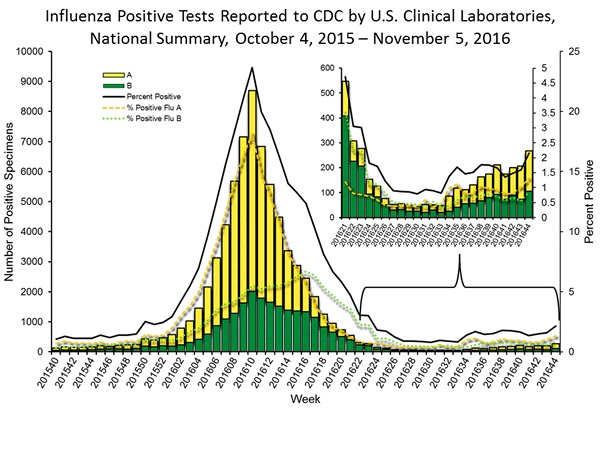
\includegraphics[scale=0.5]{WHONPHL44_small.jpg}
    \caption{Flu positive test over 2016-2017 in the U.S}
    \label{fig:my_label}
\end{figure}



\section{SIR Model}

The SIR model is a comportmental model in epidemiology and serve as a base mathematical framework of the main paper in this area. It 's help understanding complex dynamics of the spread of desease.

The model splits the population into three categories : 
\begin{enumerate}
    \item Susceptible: (denoted by S). The number of people from the population susceptible to be ill. Then vaccinated people are not susceptible.
    \item Infected: (denoted by I). The number of people from the population infected.
    \item Recovered (denoted by R) the number of people from the population recovered and immune.
    
\end{enumerate}

The dynamic of these tree variables over time can be expressed by the following differential equations:

$${\frac  {dS}{dt}}=-{\frac  {\beta IS}{N}}$$
$${\frac  {dI}{dt}}={\frac  {\beta IS}{N}}-\frac{I}{\lambda}$$
$${\frac  {dR}{dt}}=\frac{I}{\lambda}$$

$N$ is the number of people in population. We assume that the population is constant over time because the dynamic of death and birth is often slower than the dynamics of Flu.Then :
$${\frac  {dS}{dt}}+{\frac  {dI}{dt}}+{\frac  {dR}{dt}}=0$$
$\beta$ is the incidence ratio. Then $\beta I S$ is the number of people from susceptible to infected during $dt$. We can expressed $\beta$ as the product between the number of people met during $dt$ time the probability than a infected person transmits the virus to someone else.


$\lambda$ is the average number of days a person is ill. Then $\frac{I}{\lambda}$ is the flow from infected people to recovered people.


\section{Model of Flu epidemy with graph network}

Our goal is to test three models from literature and check if theya are fitted to model flu

\subsection{Pastor-Satorras and Vespignani (2001) \cite{PhysRevLett.86.3200}}

First, the model has exponential distribution.
The first result from this paper is when $\beta_{0} \Bar{k} \lambda s_0>1$ then the network will reach steady state in which $I(t) > 0$. Then we want to check if this result can be apply with flu epidemy.

Second, the edge distribution follows a Power-law degree. ($P(k) ~ k^{-\nu}$

In the same way, we want to test if flu epidemy can be modelel by Power-law degree distribution.
Then, we want to apply the result from this paper to flu epidemy in the U.S.
Here, the authors show that:
\begin{itemize}
    \item for $2<\nu<3$ the network will reach a steady state in which $I(t)>0$ for every set o f parameter values.
    \item for $3<\nu$ the infection will be endemic in the network if and only if 
    $$\beta0 \lambda > \frac{\nu-1}{m \nu}$$
\end{itemize}


\subsection{Wang et al. and Ganesh et al., (2005) \cite{wang2003epidemic,ganesh2005effect}}

Here, the authors models the network as a arbitrary network.
The result from the paper is that $\beta \lambda < \frac{1}{\lamba_A}$, where $\lambda_A$ is the largest eigenvalue.


\subsection{Watts et al., 2005 \cite{watts2005multiscale}
}

The authors use stochastic approach to model epidemic. we want to check if these approach is suited to model flu in the U.S

\section{Data}

Our project data is focus in flu epidemic in 2016-2017 in the U.S over all states.
 We have gathered data from the Centers for Disease Control and Prevention \footnote{https://www.cdc.gov/flu/} which get weekly data from flu epidemic. These data are aggregated by state and by week.
 A dynamic data vizualisation \footnote{https://gis.cdc.gov/grasp/fluview/fluportaldashboard.html} is also provided by the website.
 
 The more accurate data representing flu epidemic and how many people are infected, is the number of respiratory specimens tested (the entire population) and the number positive for influenza types A and B from this population.
 This data are collected by American laboratories\footnote{Exclusively WHO and NREVSS collaborating laboratories}
 
 Besides, we need the vaccinated ratio among population. The Centers for Disease Control and Prevention gives this ratio over week, by state and by age group.
 
 Finally, we have determined some parameters:
 \begin{itemize}
     \item $\lambda$ the number of days a people is ill is set at 2 weeks.
     \item $\beta$ is the product between the number of people met during $dt$ time the probability than a infected person transmits the virus to someone else. Then the number of people met during $dt$ is $k$, the number of edges for one nodes in the graph. We set $p_inf$ at 0.6\footnote{explication}.

The last parameters to set is $\lambda$
 \end{itemize}


\subsection{Tables}
Because tables cannot be split across pages, the best
placement for them is typically the top of the page
nearest their initial cite.  To
ensure this proper ``floating'' placement of tables, use the
environment \textbf{table} to enclose the table's contents and
the table caption.  The contents of the table itself must go
in the \textbf{tabular} environment, to
be aligned properly in rows and columns, with the desired
horizontal and vertical rules.  Again, detailed instructions
on \textbf{tabular} material
are found in the \textit{\LaTeX\ User's Guide}.

Immediately following this sentence is the point at which
Table~\ref{tab:freq} is included in the input file; compare the
placement of the table here with the table in the printed
output of this document.

\begin{table}
  \caption{Frequency of Special Characters}
  \label{tab:freq}
  \begin{tabular}{ccl}
    \toprule
    Non-English or Math&Frequency&Comments\\
    \midrule
    \O & 1 in 1,000& For Swedish names\\
    $\pi$ & 1 in 5& Common in math\\
    \$ & 4 in 5 & Used in business\\
    $\Psi^2_1$ & 1 in 40,000& Unexplained usage\\
  \bottomrule
\end{tabular}
\end{table}

To set a wider table, which takes up the whole width of the page's
live area, use the environment \textbf{table*} to enclose the table's
contents and the table caption.  As with a single-column table, this
wide table will ``float'' to a location deemed more desirable.
Immediately following this sentence is the point at which
Table~\ref{tab:commands} is included in the input file; again, it is
instructive to compare the placement of the table here with the table
in the printed output of this document.


\begin{table*}
  \caption{Some Typical Commands}
  \label{tab:commands}
  \begin{tabular}{ccl}
    \toprule
    Command &A Number & Comments\\
    \midrule
    \texttt{{\char'134}author} & 100& Author \\
    \texttt{{\char'134}table}& 300 & For tables\\
    \texttt{{\char'134}table*}& 400& For wider tables\\
    \bottomrule
  \end{tabular}
\end{table*}
% end the environment with {table*}, NOTE not {table}!

It is strongly recommended to use the package booktabs~\cite{Fear05}
and follow its main principles of typography with respect to tables:
\begin{enumerate}
\item Never, ever use vertical rules.
\item Never use double rules.
\end{enumerate}
It is also a good idea not to overuse horizontal rules.

\section{Conclusions}
This paragraph will end the body of this sample document.
Remember that you might still have Acknowledgments or
Appendices; brief samples of these
follow.  There is still the Bibliography to deal with; and
we will make a disclaimer about that here: with the exception
of the reference to the \LaTeX\ book, the citations in
this paper are to articles which have nothing to
do with the present subject and are used as
examples only.
%\end{document}  % This is where a 'short' article might terminate



 
\bibliographystyle{abbrv}

\bibliography{sample-bibliography} 

\end{document}
